\section{Writing Algorithms}\label{sec:writing_algorithms}

Some algorithms -- eg. binary search here -- don't have a linear increase in their time complexity for a linear increase to the number of elements.
For a binary search we have a \(\log(n)\) graph instead.

We don't just have to worry about time complexity though, we also have memory (storage) complexity to worry about too.

\begin{highlight}{A logarithmic graph}
    For a \(\log\) graph, the \(y\) value increases very quickly at first, before levelling off.
    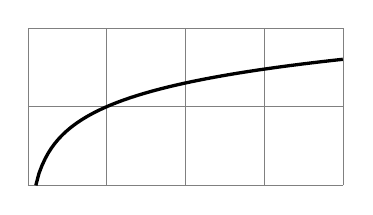
\begin{tikzpicture}
        \draw [help lines] (0, 0) grid [step=1] (4,2);
        \draw[domain=0.1:4,samples=100, very thick] plot (\x,{1 + log10(\x)});
    \end{tikzpicture}
\end{highlight}

We we need to search through unsorted data, maybe it's easier to sort the data first then store the sorted results for various searching operations later.

For sorting algorithms, there are two types of algorithm: \emph{in-place} and \emph{out-of-place} where an in-place sort doesn't create a new array, but an out-of-place one does, and therefore uses less memory.

\subsection{Planning}\label{sub:planning}

We should always plan an algorithm before we start to write it, where we clearly illustrate the final goal and all required intermediary steps.

\subsubsection{Pseudo code}\label{ssub:pseudocode}

There is no standard way of writing pseudo code, but in general instructions like \mintinline{text}{INPUT}, \mintinline{text}{OUTPUT}, \mintinline{text}{WHILE}, \mintinline{text}{FOR} and \mintinline{text}{IF} are used.

\subsubsection{Flow Charts}\label{ssub:flow_charts}

Flow charts are similar in that there is no standard way to represent them either.
A flow chart is different in that it shows the instructions as a diagram instead of a list of operations.

